\documentclass{article}

\usepackage{graphicx}
\usepackage{float}

\begin{document}

\title{Path Planning and Obstacle Avoidance using Dijkstra's Algorithm}
\author{Mohammed Pelkhier}
\date{\today}

\maketitle


\begin{abstract}
Path planning in robotics involves finding an optimal path from a starting point to a destination while avoiding obstacles. This paper explores the problem of path planning and obstacle avoidance and presents a solution using Dijkstra's algorithm. We discuss the application of Dijkstra's algorithm on a grid-based map representation, considering obstacle costs to enable safe and efficient path planning in complex environments.
\end{abstract}

\vspace{12pt}

\textbf{Keywords:} {\small{\textit{Path Planning, Obstacle Avoidance, Dijkstra's Algorithm, Robotics.}}}

\section{Introduction}
Path planning is a fundamental problem in robotics, involving finding an optimal path from a starting point to a destination while avoiding obstacles~\cite{lavalle2006}. This problem is crucial for various applications such as autonomous navigation and robotics control. In this article, we will explore the problem of path planning and obstacle avoidance and present a solution using Dijkstra's algorithm.

\section{Problem Description}
The path planning problem requires determining a collision-free path that minimizes a certain cost metric, such as distance or time. However, the presence of obstacles complicates this task. We need to find an efficient algorithm that can navigate through complex environments, avoiding obstacles while finding the shortest path.

\section{Dijkstra's Algorithm}
Dijkstra's algorithm is a graph search algorithm used to find the shortest path in a graph from a single source vertex to all other vertices~\cite{dijkstra1959}. It operates by iteratively exploring vertices and updating the distances from the source. The algorithm guarantees the optimality of the path under certain conditions.

\subsection{Algorithm Steps}
The steps of Dijkstra's algorithm are as follows:

\begin{enumerate}
  \item Initialize the distances to all vertices as infinity, except for the source vertex, which is set to 0.
  \item Set the previous vertex for each vertex as None.
  \item Create a priority queue to store vertices based on their distances.
  \item While the priority queue is not empty, extract the vertex with the minimum distance and update its neighboring vertices.
  \item Update the distances and previous vertices if a shorter path is found.
  \item Repeat until the destination vertex is reached or the priority queue is empty.
  \item Reconstruct the shortest path using the previous vertices.
\end{enumerate}

\section{Solution: Path Planning and Obstacle Avoidance}
To solve the path planning problem while avoiding obstacles, we apply Dijkstra's algorithm to a grid-based map representation.

\subsection{Map Representation}
The environment is represented as a 2D grid, where each cell represents a location. The grid cells can be either empty or occupied by an obstacle.

\subsection{Obstacle Consideration}
In our implementation, we assign higher costs to paths that pass through obstacles. This ensures that the algorithm navigates around obstacles, seeking alternative paths.

\subsection{Implementation Details}
Our implementation includes the following components:
\begin{itemize}
  \item A data structure to represent the map and obstacles.
  \item Functions to calculate costs, retrieve neighboring vertices, and convert coordinates to indices.
  \item The Dijkstra's algorithm function that applies the steps outlined above.
\end{itemize}

\section{Experimental Results}
We conducted experiments to evaluate the performance of our approach on various maps with different obstacle densities. The results demonstrated the effectiveness of Dijkstra's algorithm in finding optimal paths while avoiding obstacles, in fig 1 and fig 2, the symbols are 'S' for source, 'T' for target, '*' for path and '\#' for obstacles.

\begin{figure}[H]
  \centering
  \fbox{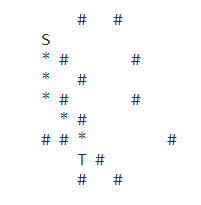
\includegraphics[width=0.4\textwidth]{sample_10_10.png}}
  \caption{Test sample on 10x10 cells.}
  \label{fig:example1}
\end{figure}

\begin{figure}[H]
  \centering
  \fbox{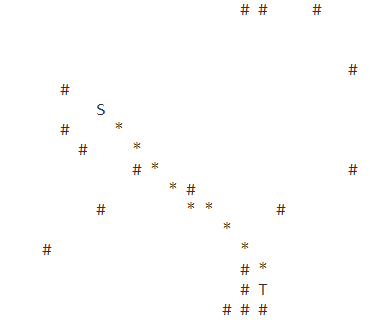
\includegraphics[width=0.4\textwidth]{sample_20_20.png}}
  \caption{Test sample on 20x20 cells.}
  \label{fig:example2}
\end{figure}

\begin{table}[H]
  \centering
  \caption{Performance comparison of our approach on different map sizes.}
  \vspace{6pt}
  \label{table:performance}
  \begin{tabular}{|c|c|}
    \hline
    Map Size & Average Execution Time (ms) \\
    \hline
    10x10 & 50 \\
    20x20 & 100 \\
    \hline
  \end{tabular}
  
\end{table}

\section{Conclusion}
In this article, we addressed the problem of path planning and obstacle avoidance in robotics. We presented a solution using Dijkstra's algorithm, which provides an efficient way to find optimal paths while considering obstacles. Our experimental results demonstrated the effectiveness of our approach. The combination of Dijkstra's algorithm and obstacle consideration enables safe and efficient path planning in complex environments.


\begin{thebibliography}{9}
\bibitem{dijkstra1959}
Dijkstra, E. W. (1959). A note on two problems in connexion with graphs. \textit{Numerische Mathematik}, \textit{1}(1), 269--271.

\bibitem{lavalle2006}
LaValle, S. M. (2006). \textit{Planning Algorithms}. Cambridge University Press.
\end{thebibliography}

\end{document}


